\begin{CJK}{Bg5}{bsmi}

%---------------------------------------------
%	Chapter System Architecture
%---------------------------------------------

\chapter{System Architecture}

In this chapter, I'll try to explain my design more detailed. First section is the basic idea of my authentication system, which is based on digital signature algorithm. The next section is about the flow if clinets and servers adopt this scheme. The next chapter gives two demonstrations of this scheme. One is for the furture website, and one if for the existing website. The last section gives a high-level code example to explain how to implement this system.

\section{Overview}

Let us recall the autehentication process about password-based scheme. As the fig\ref{fig:password-based-flow} shows, the client give his username and password to server (password is encrypted), and the server checks whether it is valid according to its database. Fig\ref{fig:my-scheme-flow} is the authentication process of my scheme. Because the verificaiton server should be a passive element, client should send a login request first. After receive a login request, the server send a random nonce back to client. Client generate a signature for this nonce and return to server. Server, then, use the public key to check whether the client is valid or not.

\begin{figure}
\centering
\subfigure[password-based scheme]{
\label{fig:password-based-flow}
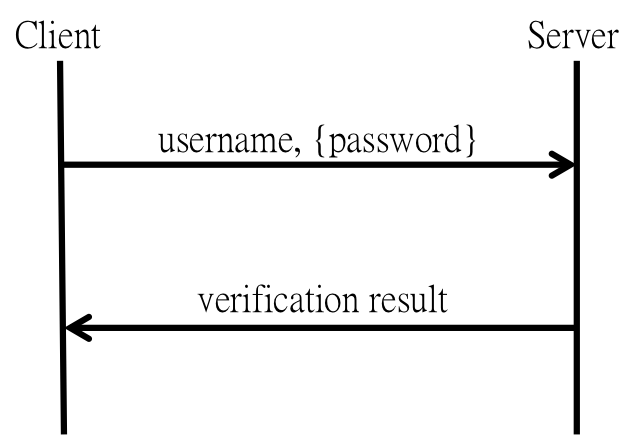
\includegraphics[scale=0.6]{picture/password-based-flow.png}
}
\subfigure[my scheme]{
\label{fig:my-scheme-flow}
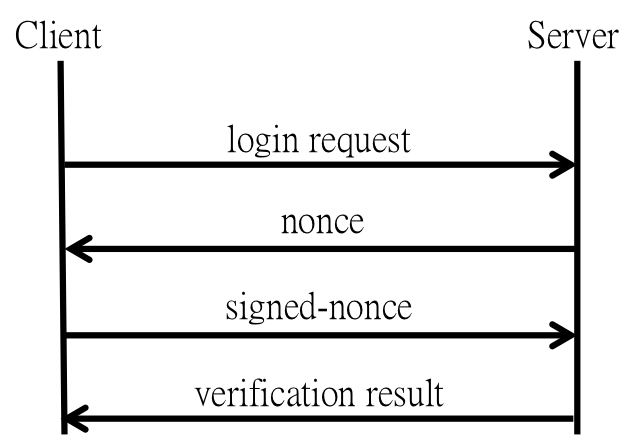
\includegraphics[scale=0.6]{picture/basic-idea-flow.png}
}
\caption{Authentication flow}
\end{figure}

This is how I used Digital Signature Algorithms in an authentication process. The advantages is that the data communicated between client and server do not need to be encrypted. The only \emph{secret} is private key, which is stored in client's storage. The disavantage of my scheme is that users will need a device to help them creating signature and manage their public keys. Therefore, the use of mobile device is the core of this scheme, bring us a high usability. The user flow become fig\ref{final-flow} with the help of mobile device.

\begin{figure}
\centering
\label{fig:final-flow}
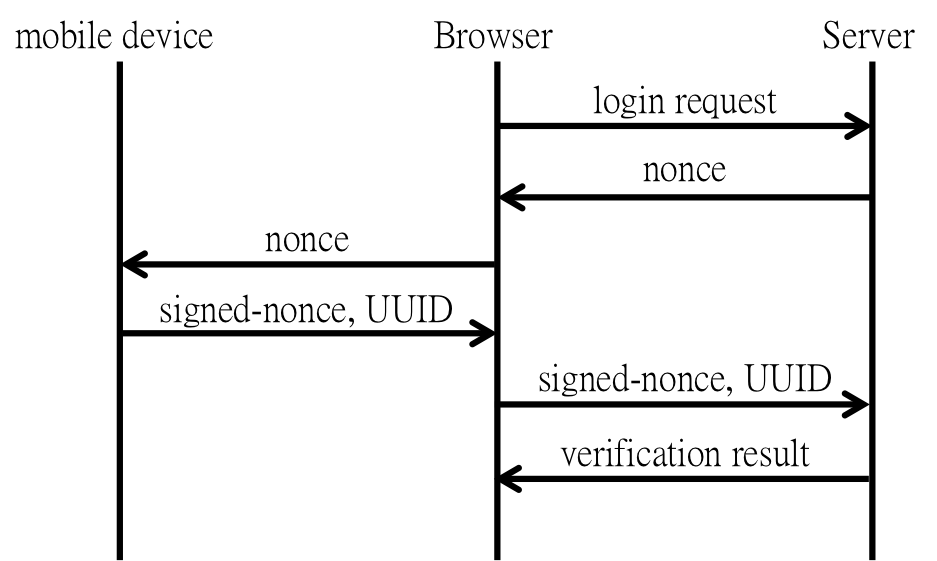
\includegraphics[scale=0.65]{picture/final-flow.png}
\caption{Authentication flow with mobile device}
\end{figure}

\section{User Flow}

In this section, I'll seperate the autentication process into three parts: \emph{register phase}, \emph{login phase} and \emph{verification phase}.

\subsubsection{Register Phase}

\begin{enumerate}
\item Start the initialzization process on his mobile device, that is, set PIN code and generate key pair.
\item User send a registration request to the verification server.
\item Server return the server information to user and pass it to mobile device via reader applicaiton.
\item Mobile device saved the server information and the private key together, and return the device UUID and corresponding public key back to user.
\item User send the id and public key (and other required credentials required by server) to server.
\item Server saved UUID and public key into its database.
\end{enumerate}

\subsubsection{Login Phase}

\begin{enumerate}
\item User send a login request to server.
\item Server return a nonce ([server info || random bits]) back to client.
\item The NFC reader start to scan cards as soon as it receive the nonce.
\item User execute the card emulation application on mobile device and enter the PIN code. If the PIN code correct, mobile device enable the HCE mode.
\item Reader application send nonce to mobile device.
\item Mobile device retrieve the server info from nonce, show it on the screen and ask for user's confirmation.
\item Mobile device signed the nonce with corresponding private key.
\item Mobile device pass its UUID and signed-nonce to reader.
\item Client pass these parameters to server.
\end{enumerate}

\subsubsection{Verification Phase}

\begin{enumerate}
\item Server retrieve the corresponding public key according to the UUID.
\item Verify the signature with the public key.
\item Return the verification result back to cient.
\end{enumerate}

\section{Scenario}

\subsection{Future Website}

\subsection{Existing Website}

\section{Implementation}

\end{CJK}